\chapter{Teoretične osnove in pregled literature}\label{cha:teorija}
Ne glede na to, ali je naloga teoretično ali eksperimentalno usmerjena, je potrebno najprej obdelati osnove obravnavane tematike. 

\section{Vir informacij}\label{sec:viri}
Pri pregledu literature naj bodo knjige in predvsem strokovni ter znanstveni članki glavni vir informacij. Pri spletnem iskanju člankov in ostale literature priporočamo uporabo naslednjih iskalnikov: Dikul, Web of Science, ScienceDirect in Google Scholar. Več o citiranju virov si preberite v nadaljevanju te predloge.

\section{Podpoglavja in slogi}\label{sec:podpoglavja}
To je primer teksta, ki sledi naslovu podpoglavja na 2.~ravni. Posamezne dele vsebine smiselno razdelite v podpoglavja, ki naj bodo ustrezno naslovljena in zaporedno oštevilčena (številčenje poglavij naj bo samodejno). Slog naslovov podpoglavij naj ustreza prednastavljenim stilom, ki so prikazani v tej predlogi in podrobno opisani v \textbf{prilogi \ref{cha:priloga}}. 

Vsako (pod)poglavje se mora začeti z uvodnim odstavkom. Podpoglavja ne smejo vsebovati samo slik, preglednic, enačb ali alinej brez ustreznega uvodnega besedila in pojasnila.

\subsection{Podpoglavje na 3.~ravni}\label{sec_podpoglavje_3}
To je primer teksta, ki sledi naslovu podpoglavja na 3.~ravni. Poglavja na 1., 2.~in 3.~ravni so številčena in se pojavijo tudi v kazalu, kar je v predlogi že nastavljeno. Uporabite lahko največ 4 ravni naslovov, pri čemer četrta raven ni oštevilčena in se ne pojavi v kazalu.

\subsubsection{Podpoglavje na 4.~ravni}
To je primer teksta, ki sledi naslovu podpoglavja na 4. ravni. Podpoglavje na 4. ravni je neoštevilčeno in se ne pojavi v kazalu, kar je v predlogi že nastavljeno.


\section{Odstavki in naštevanje}\label{sec:odstavki}
Prve vrstice odstavkov naj ne bodo zamaknjene. Med odstavke ne vrivajte dodatnih praznih vrstic. Uporaba \textbf{krepkega tiska} v besedilu je smiselna (ni pa nujna):
\begin{itemize}
\item kadar v besedilu prvič omenimo in opredelimo zelo pomemben pojem za razumevanje naloge,
\item kadar želimo posebej poudariti kakšen del ali misel,
\item kadar želimo pri naštevanju vidno ločiti posamezne dele besedila.
\end{itemize}

Kadar v besedilu uporabljamo besede iz tujih jezikov, uporabljamo poševni tisk (angl.~\emph{italic}). \underline{Podčrtanega besedila} praviloma ne uporabljamo.

Vsako naštevanje mora biti napovedano v predhodnem odstavku. Poglavje ali podpoglavje se ne začne z naštevanjem.

\subsubsection{Ravni naštevanja}
Ne glede na to, koliko hierarhičnih ravni alinej je v besedilu uporabljenih za naštevanje (običajno ne več kot 2), v celotnem besedilu vedno uporabljamo enako kombinacijo ter način označevanja posameznih ravni alinej. S tem dosežemo poenoten videz besedila. Slog za posamezen nivo alinej je že nastavljen. 

Podrobnosti sloga za 1.~in 2.~raven naštevanja so opisane v \textbf{prilogi \ref{cha:priloga}}.
\begin{itemize}
\item primer 1.~ravni naštevanja:
\begin{itemize}
\item primer 2.~ravni naštevanja,
\item primer 2.~ravni naštevanja,
\end{itemize}
\end{itemize}
Med alineje in pred novim odstavkom besedila za zadnjo alinejo ne vstavljajte praznih vrstic.


\subsection{Preglednice}\label{sec:preglednice}
Preglednice naj imajo vstavljene napise z izbranim ustreznim stilom, naj bodo zaporedno oštevilčene in oblikovane, kot to opredeljujejo navodila v \textbf{prilogi \ref{cha:priloga}}. Preglednice in njihovi napisi naj bodo levo poravnani. Med besedilom pred preglednico, napisom preglednice in preglednico ne vstavljajte dodatnih praznih vrstic.

Napis preglednice naj se začne z veliko začetnico in konča s končnim ločilom, kot je to prikazano na primeru preglednice \ref{tab:ucinkovitost}. Napis naj bo dovolj poveden, da je vsebino preglednice možno razumeti kot samostojen element.

Preglednica naj bo smiselno umeščena v besedilo. Običajno preglednico umestimo pod odstavek, v katerem preglednico prvič omenimo in jo navedemo s številko preglednice. Če preglednico zaradi bolj tekočega oblikovanja besedila umestimo drugače, naj bo umeščena v bližini prve omembe v besedilu, vendar za prvo omembo. Preglednica ne sme biti umeščena pred besedilom na začetku poglavja/podpoglavja. Pri sklicevanju na preglednice in druge dele besedila sledite navodilom, ki so opisani v \textbf{prilogi \ref{cha:priloga}}.

\begin{table}[htbp]
	\caption{Učinkovitost procesov odstranjevanja različnih onesnaževalcev vode.}\label{tab:ucinkovitost}
	\setlength{\tabcolsep}{4pt}
	\renewcommand{\arraystretch}{1.3}
\begin{tabular}{@{}>{\raggedright\arraybackslash}m{52mm}
		*{4}{>{\centering\arraybackslash}m{22mm}}@{}}
	\toprule
	\multicolumn{1}{@{}>{\centering\arraybackslash}m{52mm}}{Proces}
	& Odstranitev mikroorganizmov
	& Odstranitev suspendiranih snovi
	& Odstranitev raztopljenih anorganskih snovi
	& Odstranitev raztopljenih organskih snovi \\
	\midrule
	\textbf{Biološki} & & & & \\
	\hspace{3mm}Aktivno blato              & $+$ & $+$ & $-$ & $+$ \\
	\hspace{3mm}Anaerobna obdelava         & $-$ & $+$ & $-$ & $+$ \\
	\hspace{3mm}Biofiltri                  & $-$ & $-$ & $-$ & $+$ \\
	\addlinespace[2pt]
	\textbf{Fizikalni} & & & & \\
	\hspace{3mm}Adsorpcija na aktiv.\ oglju: & & & & \\
	\hspace{7mm}v granulah                 & $-$ & $+$ & $-$ & $+$ \\
	\hspace{7mm}v prahu                    & $+$ & $+$ & $-$ & $+$ \\
	\hspace{3mm}Konvencionalna filtracija  & $-$ & $+$ & $-$ & $-$ \\
	\hspace{3mm}Flokulacija + sediment.    & $+$ & $+$ & $-$ & $-$ \\
	\hspace{3mm}Membranski procesi & & & & \\
	\hspace{7mm}MF                         & $+$ & $+$ & $-$ & $-$ \\
	\bottomrule
\end{tabular}
{\fontsize{8}{9.6}\selectfont Legenda: $+$ odstranjevanje poteka učinkovito, o~odstranjevanje delno poteka, $-$ odstranjevanje ne poteka}
\end{table}

Če je preglednica ali del preglednice povzet iz drugega vira, ga je potrebno citirati, kot je to prikazano na primeru preglednice \ref{tab:poraba}. Če je povzeta celotna preglednica, se številko reference napiše k napisu preglednice. Če so povzete le določene vrednosti ali besedilo znotraj celic, se to lahko citira v posameznih celicah ali na koncu posamezne vrstice.

\begin{table}[htbp]
	\caption{Kumulativne vrednosti porabe vode na vseh filtracijskih enotah za leto 2012 \cite{grote2021}.}\label{tab:poraba}
	\setlength{\tabcolsep}{4pt}
	\renewcommand{\arraystretch}{1.3}
\begin{tabular*}{\textwidth}{@{\extracolsep{\fill}}l*{7}{c}@{}}
	\toprule
	& $V_\mathrm{f}$
	& $V_\mathrm{sp} + V_\text{kč,sp}$
	& $V_\mathrm{v}$
	& $V_\mathrm{p,cel}$
	& $V_\mathrm{pov} + V_\text{kč,pov}$
	& $V_\mathrm{p}$
	& $\varepsilon_\mathrm{UF}$ \\
	Mesec & [m$^3$] & [m$^3$] & [m$^3$] & [m$^3$] & [m$^3$] & [m$^3$] & [\%] \\
	\midrule
	Januar    & 34785 & 2315 & 37100 & 34785 & 9192 & 25593 & 69,0 \\
	Februar   & 28575 & 1574 & 30149 & 28575 & 8743 & 19832 & 65,8 \\
	Marec     & 34002 & 1517 & 35519 & 34002 & 8963 & 25039 & 70,5 \\
	April     & 32118 &  882 & 33081 & 32118 & 7516 & 24602 & 74,4 \\
	Maj       & 33949 &  548 & 34497 & 33949 & 7457 & 26492 & 76,8 \\
	Junij     & 37004 &  137 & 37141 & 37004 & 7175 & 29966 & 80,7 \\
	Julij     & 34276 &  455 & 34731 & 34276 & 7145 & 27131 & 78,1 \\
	Avgust    & 15621 &  834 & 16455 & 15621 & 3200 & 12421 & 75,5 \\
	September & 29969 &  595 & 30564 & 29969 & 7937 & 22032 & 72,1 \\
	Oktober   & 31468 &  764 & 32232 & 31468 & 8242 & 23226 & 72,1 \\
	November  & 29033 & 1143 & 30176 & 29033 & 8065 & 20968 & 69,5 \\
	December  & 31874 & 1260 & 33134 & 31874 & 7463 & 24411 & 73,7 \\
	\bottomrule
\end{tabular*}
\end{table}


\subsection{Slike}\label{sec:slike}
Slike morajo biti zaporedno oštevilčene in oblikovane, kot to opredeljujejo navodila v \textbf{prilogi \ref{cha:priloga}}. Slike in njihovi napisi naj bodo sredinsko poravnani, kot to prikazuje primer slike \ref{fig:tekstura}. Praznih vrstic med odstavkom pred sliko, napisom slike in odstavkom za sliko ne vstavljajte.

Napis slike naj se začne z veliko začetnico in konča s končnim ločilom. Napis naj bo dovolj poveden, da je vsebino slike možno razumeti kot samostojen element. Slike morajo biti dobre kakovosti in v slovenskem jeziku.

\begin{figure}[htbp]
	\centering
	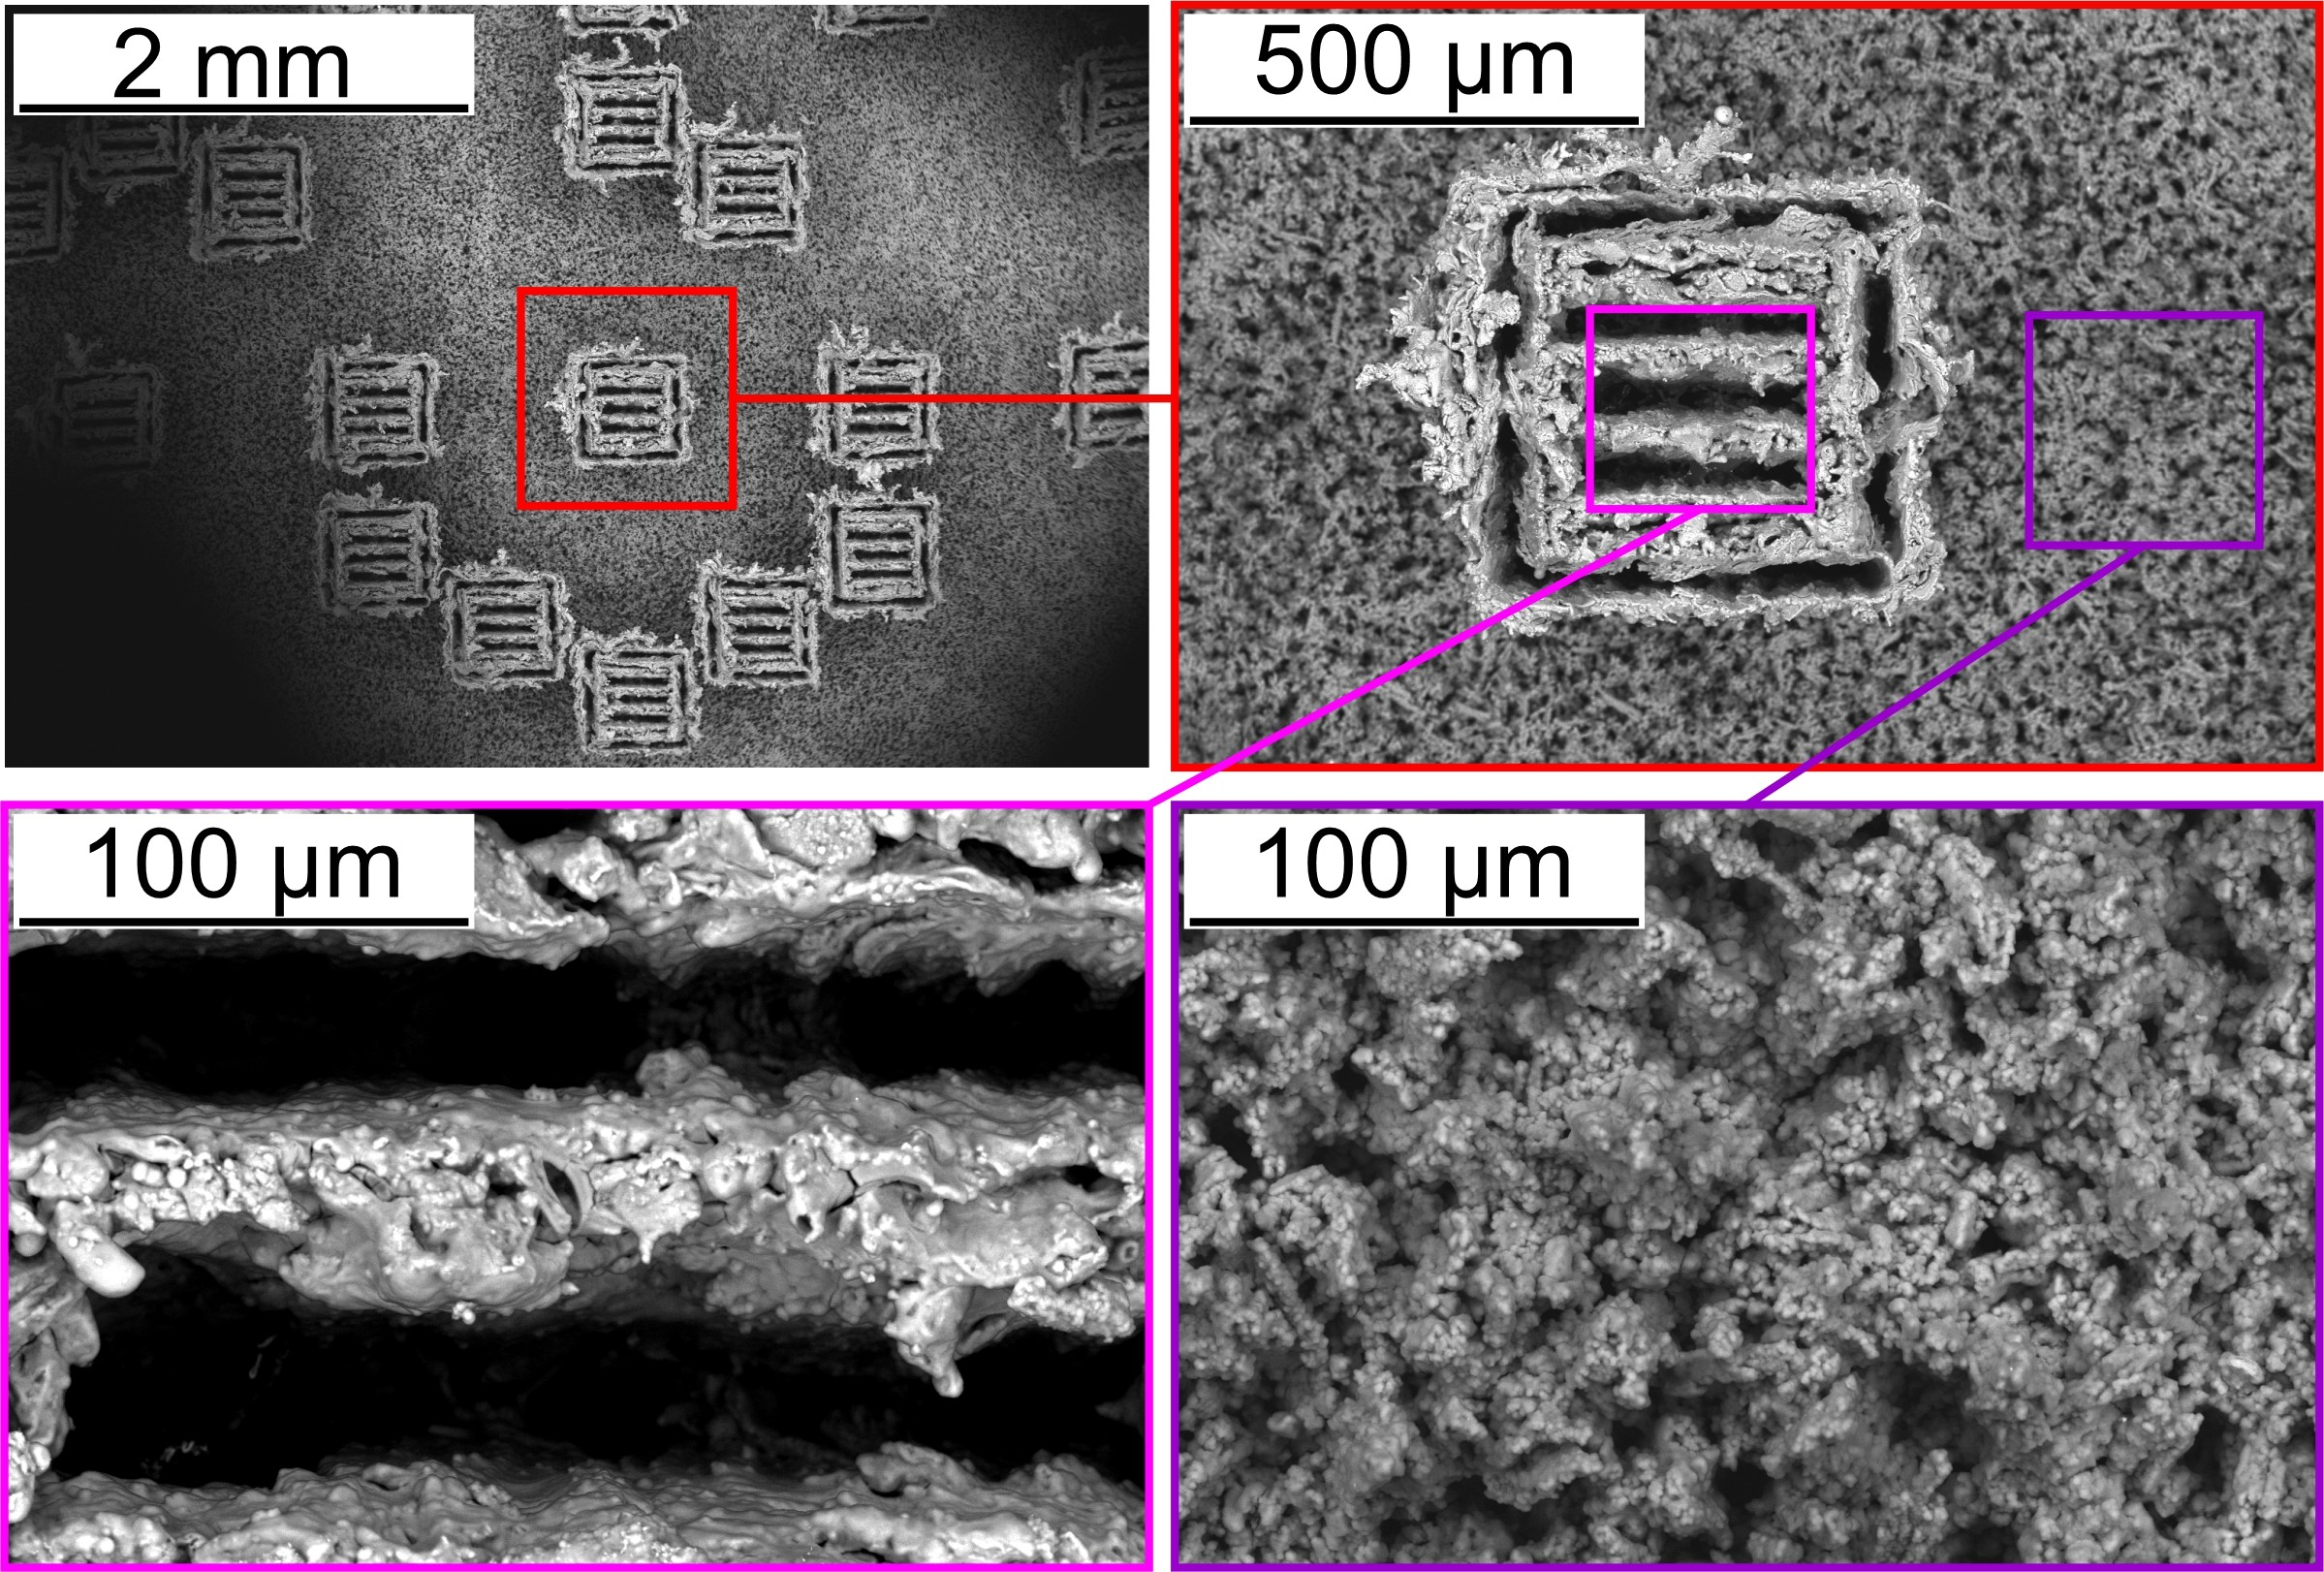
\includegraphics[width=101.5mm]{slike/tekstura.jpg}
	\caption{Lasersko teksturiran in kemično jedkan aluminijev vzorec, posnet z vrstičnim elektronskim mikroskopom \cite{grote2021}.}\label{fig:tekstura}
\end{figure}

Vsaka slika (npr. slika \ref{fig:polimerizacija} ali \ref{fig:diagrami}) naj bo pred pojavitvijo s številko omenjena v besedilu in tudi širše pojasnjena. Običajno sliko umestimo pod odstavek, v katerem jo prvič omenimo. Če sliko zaradi bolj tekočega oblikovanja besedila umestimo drugače, naj bo umeščena v bližini prve omembe v besedilu, vendar za prvo omembo. Slika ne sme biti umeščena pred besedilom na začetku poglavja/podpoglavja. Pri sklicevanju na slike in druge dele besedila sledite navodilom, ki so opisani v \textbf{prilogi \ref{cha:priloga}}.

\begin{figure}[htbp]
	\centering
	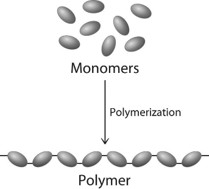
\includegraphics[width=55.2mm]{slike/polimeri.jpg}
	\caption{Shematski prikaz postopka polimerizacije s primerom prevoda tujih izrazov na izvirni sliki v slovenščino \cite{bower2025,stephan2021}.}\label{fig:polimerizacija}
\end{figure}

Če je slika ali del slike povzet iz drugega vira, ga je potrebno citirati, kot je to prikazano na primeru slik \ref{fig:tekstura} in \ref{fig:polimerizacija}. Če je na sliki diagram, morajo biti veličine in enote vseh osi jasno in dosledno označene. Pri razmejevanju naslova osi in enot uporabite enoten stil v celotni nalogi (tako na slikah, v enačbah in v besedilu naloge). Imenu osi na diagramih naj sledi oznaka veličine in enote, ki jih zapišite v oglatem ali okroglem oklepaju (vseskozi uporabljaje zgolj en način). Primer prikazuje slika \ref{fig:diagrami}.

\begin{figure}[htbp]
	\centering
	\begin{subfigure}[b]{77mm}
		\centering
		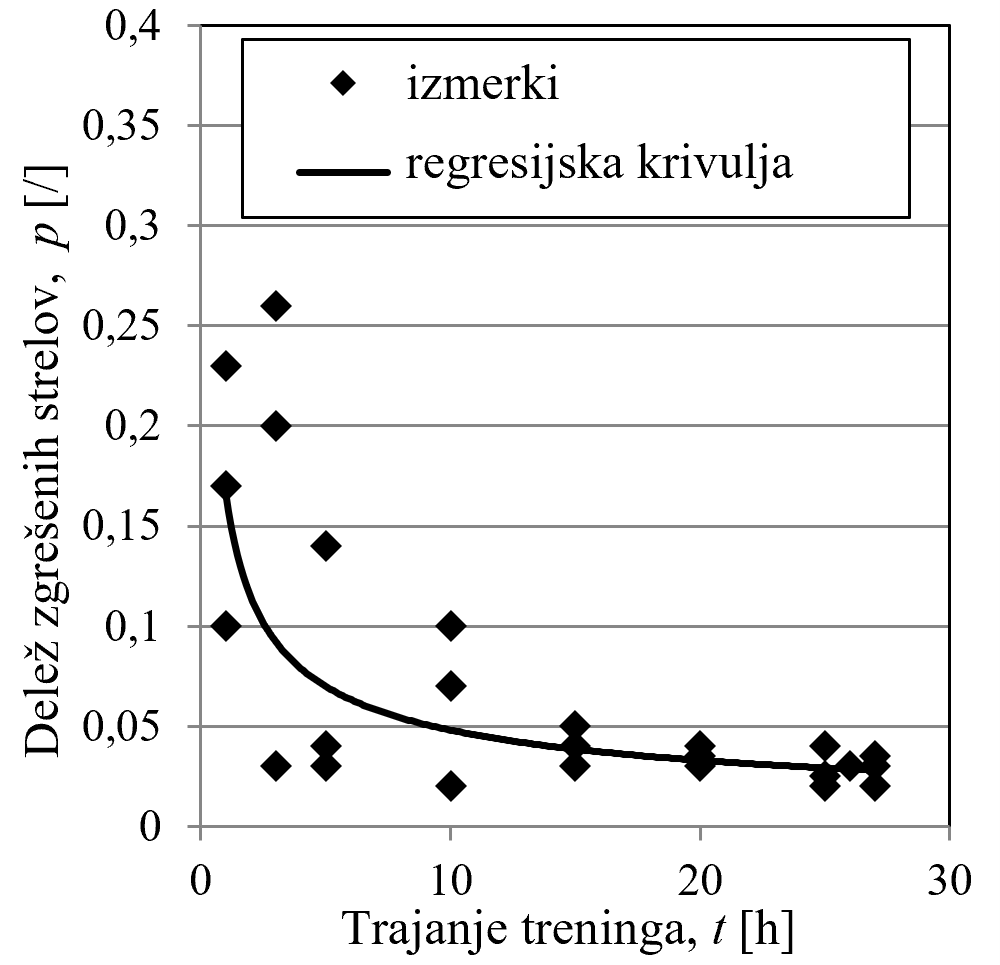
\includegraphics[width=\linewidth]{slike/streli_a.png}
		\caption{}\label{fig:diagrami_a}
	\end{subfigure}\hfill
	\begin{subfigure}[b]{77mm}
		\centering
		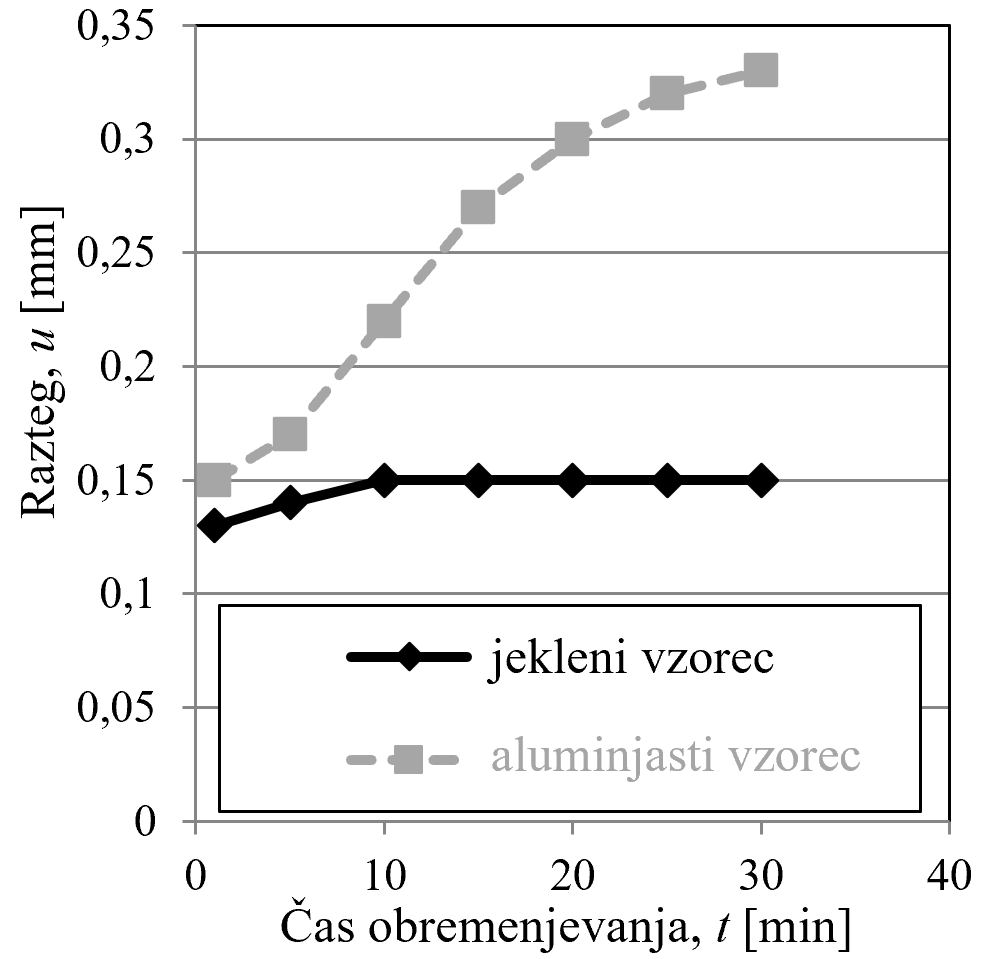
\includegraphics[width=\linewidth]{slike/streli_b.png}
		\caption{}\label{fig:diagrami_b}
	\end{subfigure}
	\caption{(a) Odvisnost deleža zgrešenih strelov na tekmovanju v odvisnosti od časa treninga pred njim. (b) Deformacija v odvisnosti od časa obremenjevanja za dva različna vzorca.}\label{fig:diagrami}
\end{figure}

Na mikroskopskih posnetkih mora biti ustrezno označena dolžinska skala, kot to prikazuje slika \ref{fig:tekstura}. Pri zaporedju časovno razmejenih slik naj bodo označeni relativni časi, kot to prikazuje slika \ref{fig:padec}.

\begin{figure}[htbp]
	\centering
	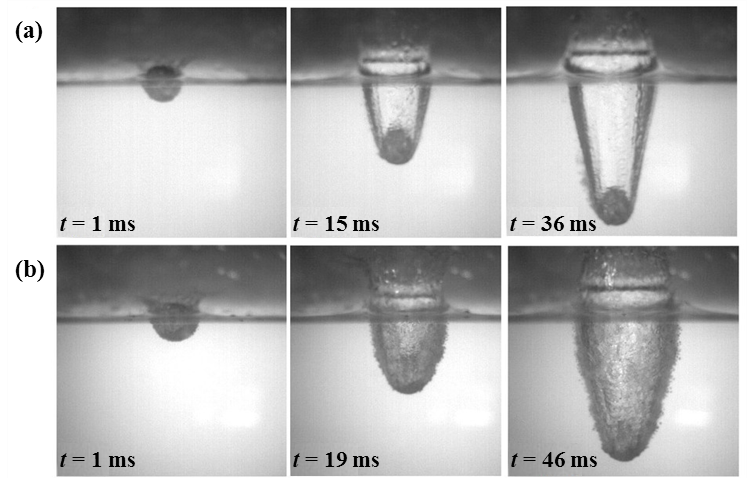
\includegraphics[width=126.5mm]{slike/mikroskop.png}
	\caption{Časovno sosledje padca projektila v vodo z višine (a) 2,1~m; in (b) 4,1~m \cite{tsao1993}.}\label{fig:padec}
\end{figure}

Kot je prikazano na slikah \ref{fig:diagrami} in \ref{fig:padec}, lahko več povezanih delov slike združite v eno sliko, pri čemer jih jasno ločite na podsklope, tj. (a), (b),\ldots{} Pri tem pazite na preglednost. Posamezni podsklopi morajo biti obrazloženi v napisu slike. Pri sklicevanju na posamezen podsklop slike v besedilu naloge to storite z navedbo črke v oklepaju takoj za številko slike, npr. slika \ref{fig:padec}(b).

\section{Enačbe}\label{sec:enacbe}
Za vnos enačbe uporabljajte način \verb|equation|. To bo samodejno vstavilo enačbo s samodejnim oštevilčenjem okroglem oklepaju.

Enačbo nato prilagodite in po potrebi posodobite zaporedno številko enačbe v poglavju. Podrobna navodila glede vstavljanja in oblikovnega izgleda enačb so navedena v \textbf{prilogi \ref{cha:priloga}}.

V nadaljevanju so prikazani primeri enačb. Številčenje se začne s številko prve ravni poglavja, v katerem se enačba nahaja, sledi zaporedna številka enačbe v tem poglavju. Pojasnilo enačbe in veličin, ki se v enačbi pojavijo prvič, mora biti v besedilu naloge.

To je primer matematičnega zapisa drugega Newtonovega zakona
\begin{equation}\label{eq:F}
	\bm{F}=m\bm{a},
\end{equation}
kjer so $\bm{F}$ sila, $m$ masa telesa in $\bm{a}$ pospešek telesa. Enačba, ki je vstavljena v poved, se konča z ločilom, če je to potrebno. Enačba, ki stoji samostojno, ločila ne potrebuje. Dva primera enačb sta:
\begin{equation}\label{eq:e}
	e=mc^2
\end{equation}
in
\begin{equation}\label{eq:ecel}
	e_\mathrm{cel}=\sum_{i=1}^{n} m_i c^2.
\end{equation}
Pri tem je $e$ energija delca, $c$ je svetlobna hitrost in $e_\mathrm{cel}$ je energija celotnega sistema.

V besedilu, če je to potrebno, se sklicuje na ustrezno številko enačbe s celo besedo, npr.~na enačbo \eqref{eq:F}. Navodila za dodajanje sklicev na določena dela besedil ali elementov so opisana v \textbf{prilogi \ref{cha:priloga}}.

\subsection{Oznake veličin}\label{sec:oznake_velicin}
Za oznake veličin in druge simbole običajno uporabljamo črke latinske in grške abecede, včasih z dodatki indeksov in drugih znakov. Kot je prikazano v enačbah \eqref{eq:F}--\eqref{eq:ecel}, morajo biti simboli, torej oznake skalarnih veličin, npr.~$e$ ali $m$, pisane v poševnem tisku, vektorske in tenzorske (matrične) veličine, npr.~sila $\bm{F}$, pa morajo biti pisane v poševnem in krepkem tisku. Pri tem oblikovanju sledite pravilom standarda ISO 80000.

Indekse običajno uporabimo, kadar imata dve veličini enak simbol, ali pa če želimo veličino dodatno opredeliti (npr.~$_\mathrm{dop}$ kot dopustni, $_\mathrm{cel}$ kot celoten, $_\mathrm{z}$ kot začetni itn.). Če so ti indeksi opisni, se pišejo pokonci.

Indekse, ki označujejo fizikalne veličine, pišemo v poševnem tisku, npr.~$c_p$, ki predstavlja specifično toploto pri konstantnem tlaku.

Indeksi, ki opisujejo mesta v zaporedju, v matriki itn., se pišejo poševno. Tak primer je $\bm{F}_i$, kjer to pomeni $i$-to silo ali $\bm{A}_{ij}$, kjer to pomeni element $i$-te vrstice in $j$-tega stolpca v matriki $\bm{A}$.


\section{Citiranje in navajanje virov}\label{sec:citiranje}
Pri citiranju upoštevajte pravila citiranja, ki ne veljajo le za zaključna dela, temveč tudi v splošnem za vsako predstavitev, v kateri sta uporabljeni intelektualna ali materialna lastnina drugih avtorjev. Kot vire v čim večji meri uporabljajte novejšo relevantno mednarodno strokovno literaturo. Spletni viri lahko predstavljajo \textbf{največ 25~\%} vseh virov, uporabljenih v zaključnem delu. Vsi spletni viri morajo imeti v seznamu literature naveden datum zadnjega ogleda.

Vso uporabljeno literaturo v besedilu morate navajati sproti po zaporednih številkah v \textbf{oglatem oklepaju}, zato naj bo tudi popis bibliografije oštevilčen v skladu z zaporedjem pojavljanja citatov v dokumentu. Različni primeri ustreznega navajanja literature so prikazani v naslednjem odstavku.

V delu Zhang et al.~\cite{zhang2025} je podan pregled vplivov površinske obdelave na delovanje zobniške dvojice. V prispevku \cite{zhang2025} je podan pregled vplivov površinske obdelave na delovanje zobniške dvojice.

V kolikor se trditev ali informacija, ki jo navajate, nanaša na več virov, je potrebno te navesti znotraj enega oglatega oklepaja po naraščajočih številkah. Na primer \cite{grote2021,bower2025}, \cite{grote2021,bower2025,stephan2021,tsao1993} ali \cite{grote2021,stephan2021,zhang2025,zibert2025,niculuta2012,gyroid,dawkins,znidarsic2025,merkur2005,surs2009,zgd1,iso690}. Če uporabljate LaTeX, se združevanje referenc izvede avtomatsko.

V kolikor dobesedno navajate daljši odsek besedila iz drugega vira, ga označite z navednicami. Na primer, 70.c člen Zakona o gospodarskih družbah pri poročanju o trajnostnosti med drugim zahteva »\ldots{}opis časovno vezanih ciljev glede zadev v zvezi s trajnostnostjo, ki jih določi družba, kadar je to glede na evropske standarde poročanja o trajnostnosti potrebno, vključno s cilji glede absolutnega zmanjšanja emisij toplogrednih plinov vsaj za leti 2030 in 2050\ldots« \cite{zgd1}.

Zaporedna številka vira, na katerega se sklicujemo v oglatem oklepaju, se ponovi v popisu literature. Vzorci popisa literature so navedeni v \textbf{prilogi \ref{cha:priloga}}. Pri kasnejšem ponovnem sklicevanju na isto referenco uporabimo enako številko kot pri prvem sklicu.